\chapter{Monte Carlo Simulations}
\label{app:montecarlo}

All Monte Carlo simulations performed in this thesis are listed in this appendix chapter.
The Monte Carlo simulations were performed by first simulating a trajectory, using the motion model.
The model state velocity and angular velocity were also driven by Gaussian process noise in order to not simulate a perfect trajectory.
The trajectory was estimated with generated measurements plus Gaussian measurement noise in order to simulate ''real-world'' measurements.
The estimated states were then compared to the simulated states by calculating the \abbrRMSE.
A comparison of the estimated variance from the \abbrEKF and the mean-square error (\abbrMSE) were also performed.

Here, some additional figures to the once presented in \Chapterref{cha:result} will be shown.

In \Figureref{fig:27montesimstraighttowardsroitrajpos} and \Figureref{fig:27montesimstraighttowardsroitrajother}, one example of a trajectory from the Monte Carlo simulations in \Figureref{fig:27montesimstraighttowardsroirmse} is shown.

In \Figureref{fig:20montesimstraighttowardsroiangveltrajpos} and \Figureref{fig:20montesimstraighttowardsroiangveltrajother}, one example of a trajectory from the Monte Carlo simulations in \Figureref{fig:20montesimstraighttowardsroiangvelrmse} is shown.

In \Figureref{fig:30montesimstraighttowardsroiangvelcornertrajpos} and \Figureref{fig:30montesimstraighttowardsroiangvelcornertrajother}, one example of a trajectory from the Monte Carlo simulations in \Figureref{fig:30montesimstraighttowardsroiangvelcornerrmse} is shown.

In \Figureref{fig:13trajectorycrossingroipos} and \Figureref{fig:13trajectorycrossingroiother}, one example of a trajectory from the Monte Carlo simulations in \Figureref{fig:13montesimcrossingroirmse} is shown.

In \Figureref{fig:23trajectorycrossingroiangvelpos} and \Figureref{fig:23trajectorycrossingroiangvelother}, one example of a trajectory from the Monte Carlo simulations in \Figureref{fig:23montesimcrossingroiangvelrmse} is shown.

In \Figureref{fig:29trajectorycrossingroiangvelcornerpos} and \Figureref{fig:29trajectorycrossingroiangvelcornerother}, one example of a trajectory from the Monte Carlo simulations in \Figureref{fig:29montesimcrossingroiangvelcornerrmse} is shown.

\begin{figure}[!ht]
	\centering
	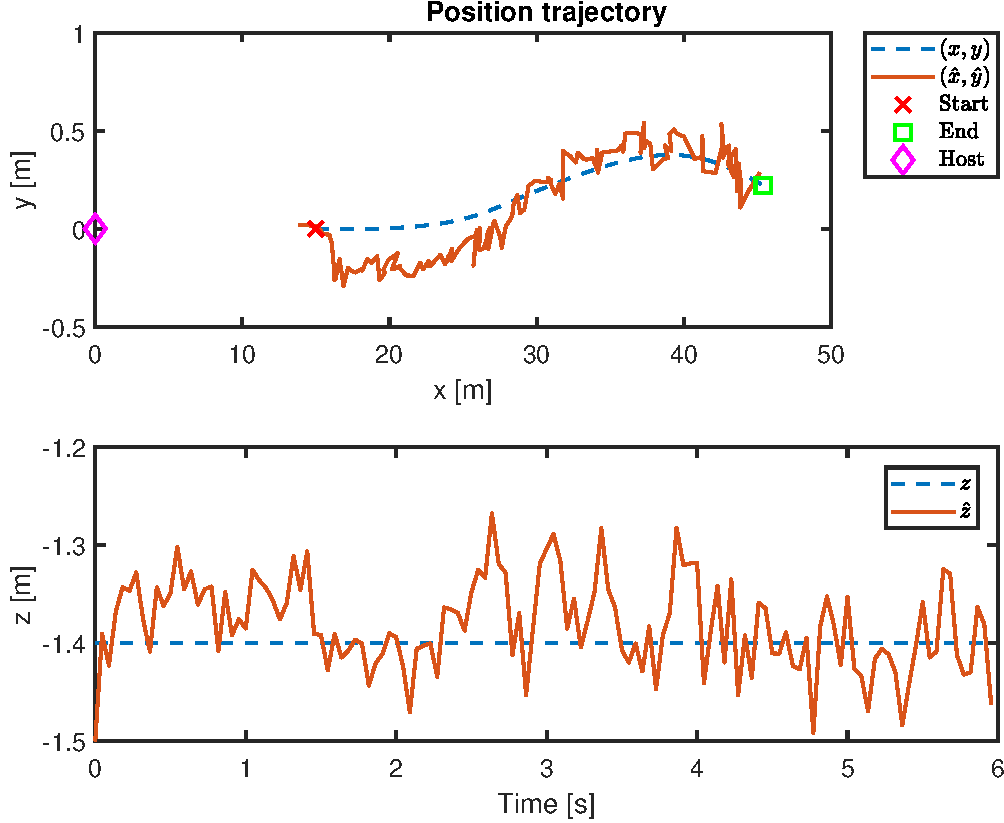
\includegraphics[width=0.8\textwidth]{ExampleTrajectory/27_MC_TrajPos}
	\caption{\label{fig:27montesimstraighttowardsroitrajpos} One example of a trajectory from the Monte Carlo simulation in scenario 1 with setup 1.}
\end{figure}

\begin{figure}[!ht]
	\centering
	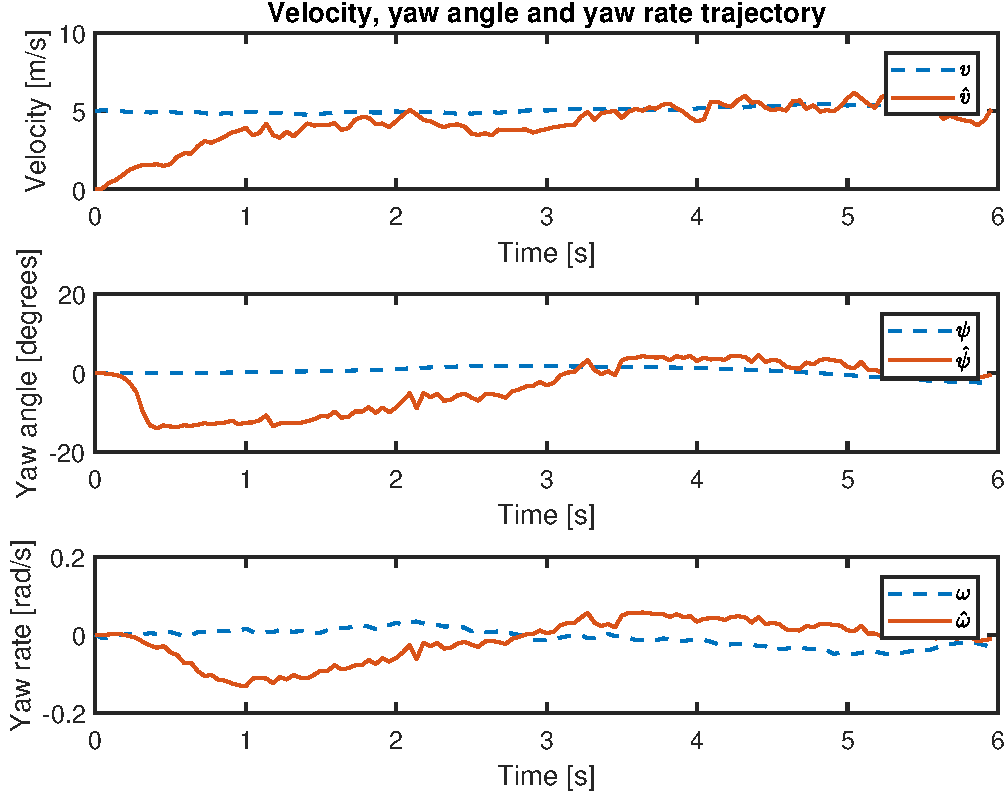
\includegraphics[width=0.8\textwidth]{ExampleTrajectory/27_MC_TrajOther}
	\caption{\label{fig:27montesimstraighttowardsroitrajother} One example of a trajectory from the Monte Carlo simulation in scenario 1 with setup 1.}
\end{figure}

\begin{figure}[!ht]
	\centering
	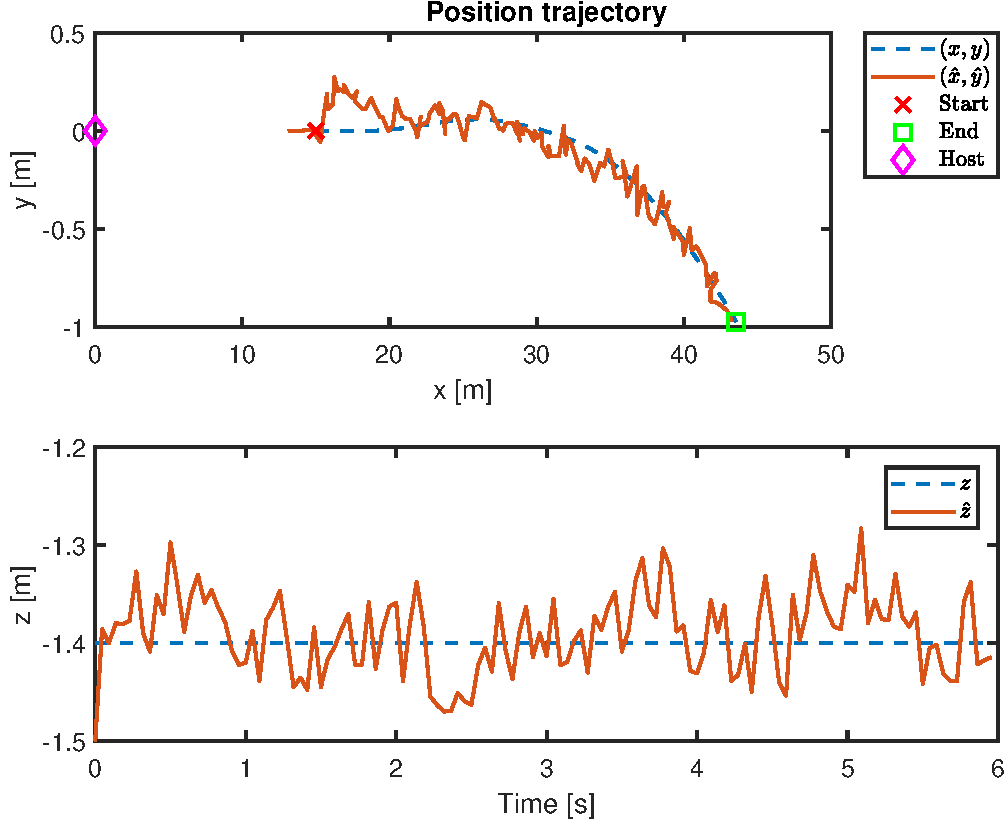
\includegraphics[width=0.8\textwidth]{ExampleTrajectory/20_MC_TrajPos}
	\caption{\label{fig:20montesimstraighttowardsroiangveltrajpos} One example of a trajectory from the Monte Carlo simulation in scenario 1 with setup 2.}
\end{figure}

\begin{figure}[!ht]
	\centering
	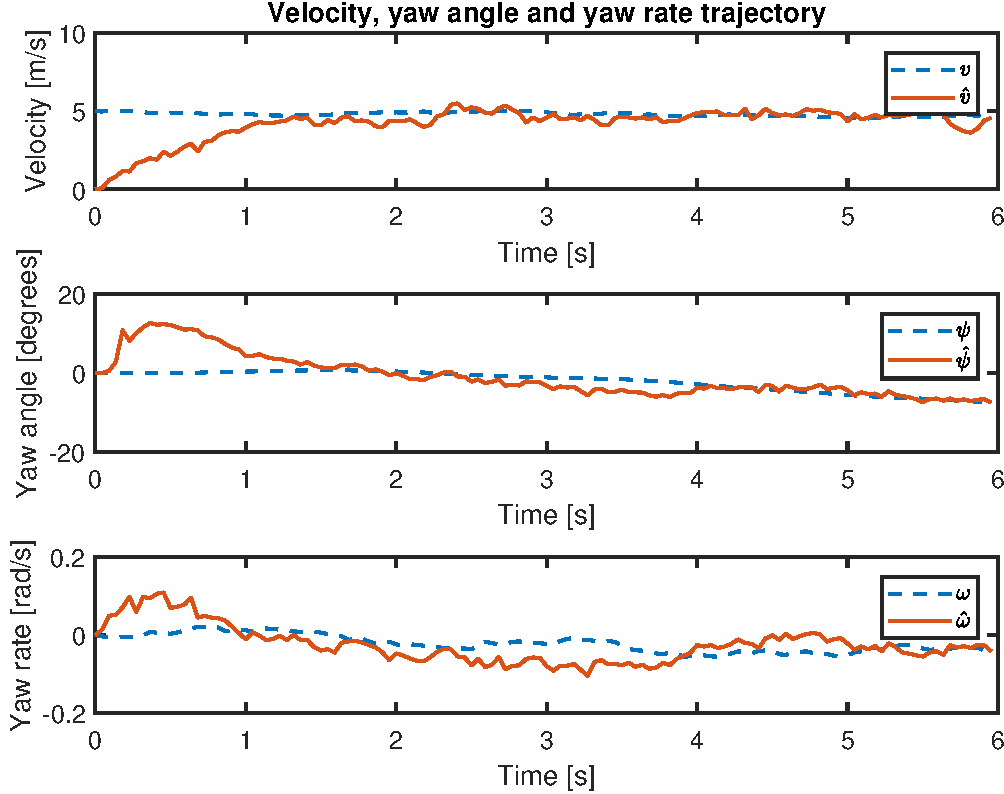
\includegraphics[width=0.8\textwidth]{ExampleTrajectory/20_MC_TrajOther}
	\caption{\label{fig:20montesimstraighttowardsroiangveltrajother} One example of a trajectory from the Monte Carlo simulation in scenario 1 with setup 2.}
\end{figure}

\begin{figure}[!ht]
	\centering
	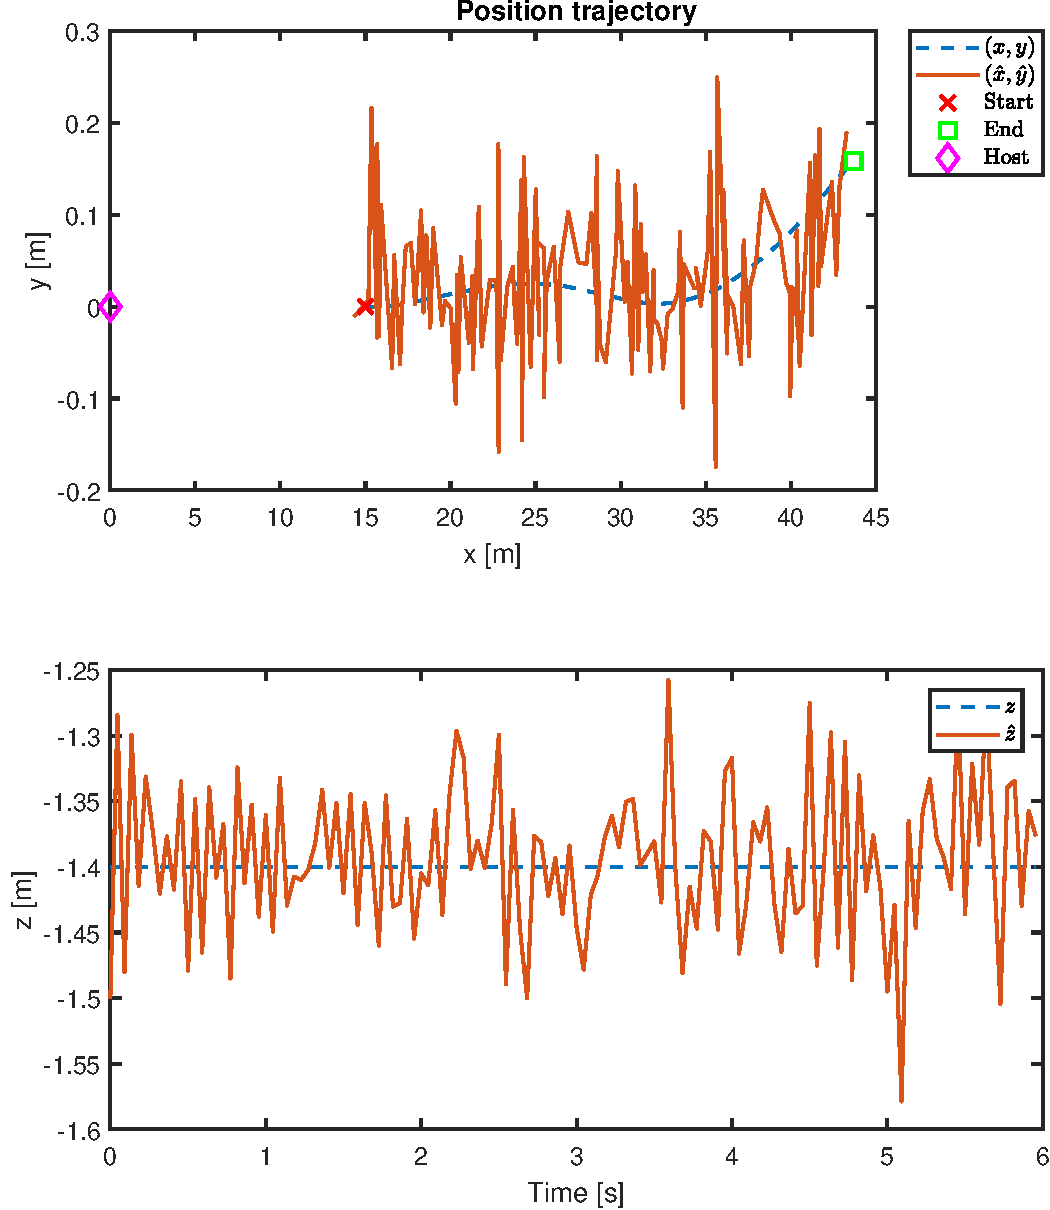
\includegraphics[width=0.6\textwidth]{ExampleTrajectory/30_MC_TrajPos}
	\caption{\label{fig:30montesimstraighttowardsroiangvelcornertrajpos} One example of a trajectory from the Monte Carlo simulation in scenario 1 with setup 5.}
\end{figure}

\begin{figure}[!ht]
	\centering
	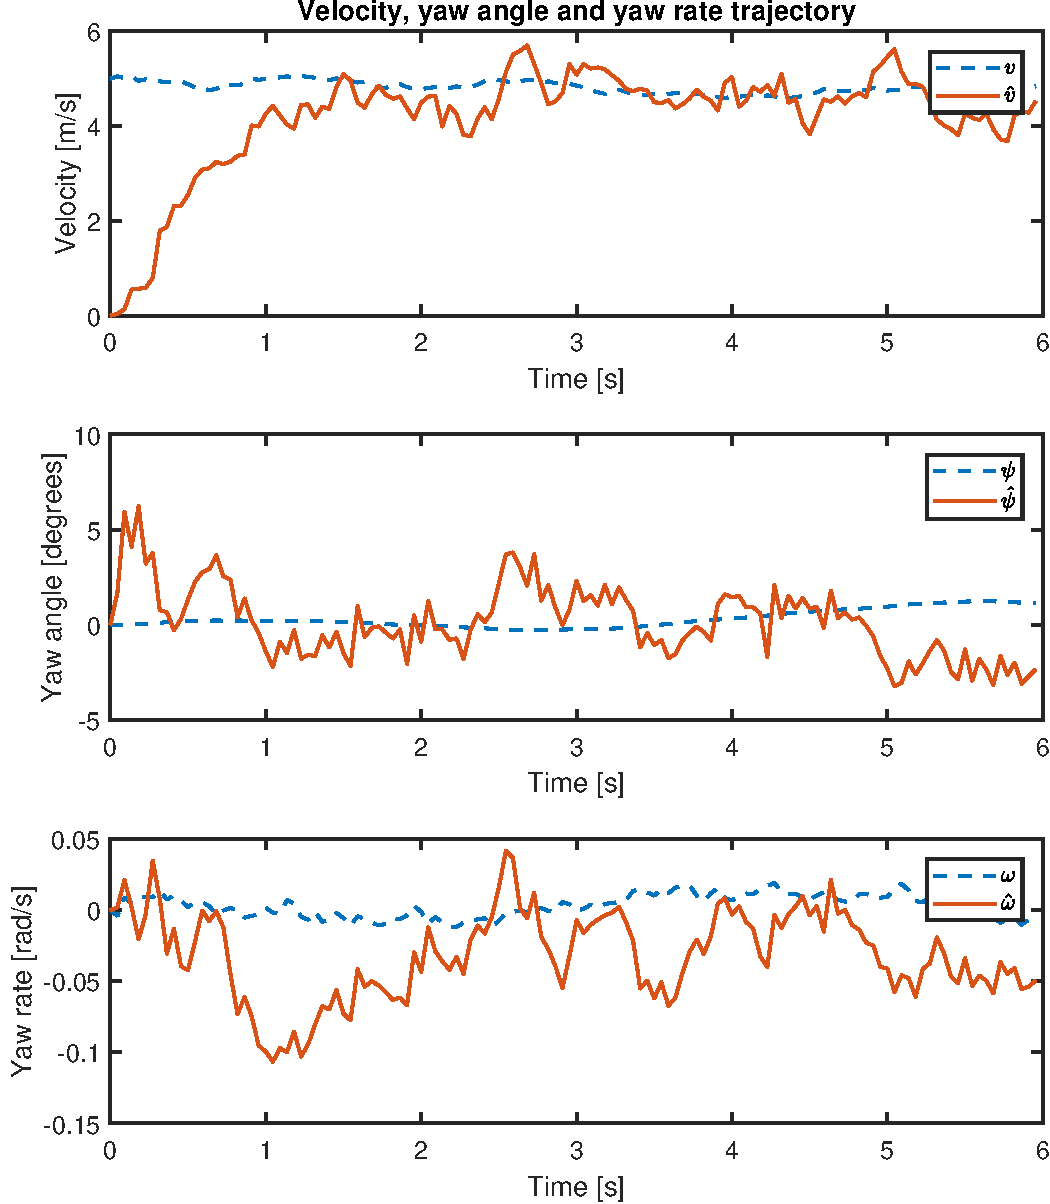
\includegraphics[width=0.5\textwidth]{ExampleTrajectory/30_MC_TrajOther}
	\caption{\label{fig:30montesimstraighttowardsroiangvelcornertrajother} One example of a trajectory from the Monte Carlo simulation in scenario 1 with setup 5.}
\end{figure}

\begin{figure}[!ht]
	\centering
	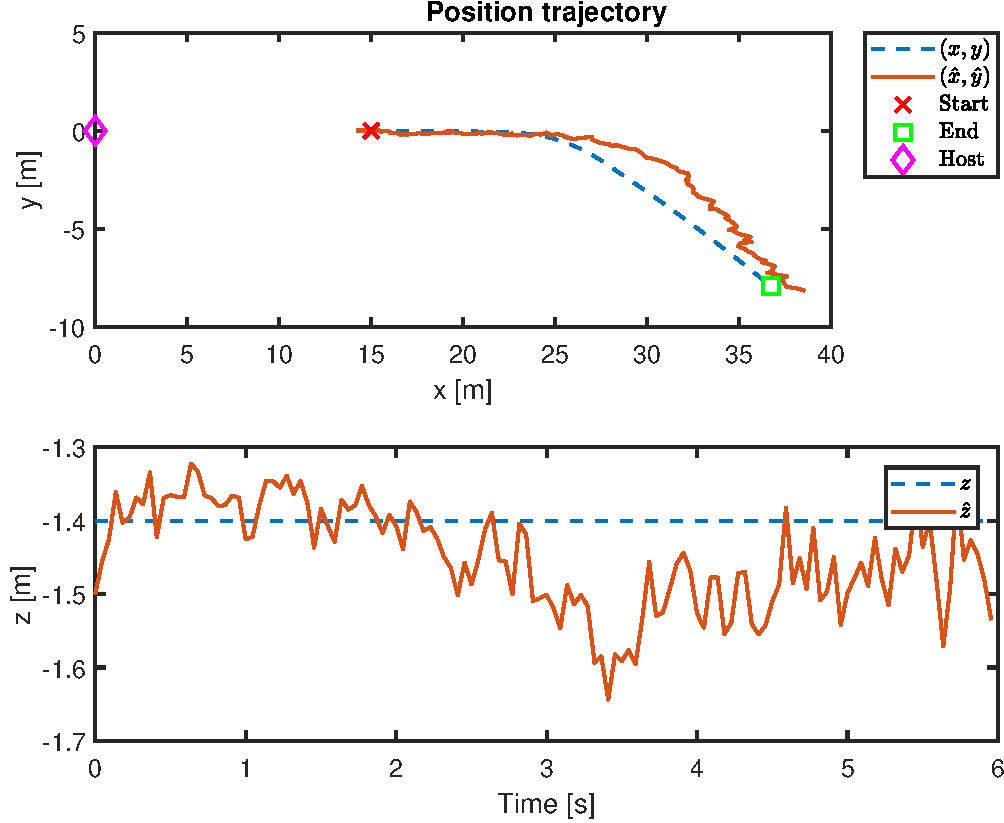
\includegraphics[width=0.8\textwidth]{ExampleTrajectory/13_MC_TrajPos}
	\caption{\label{fig:13trajectorycrossingroipos} One example of a trajectory from the Monte Carlo simulation in scenario 2 with setup 6.}
\end{figure}

\begin{figure}[!ht]
	\centering
	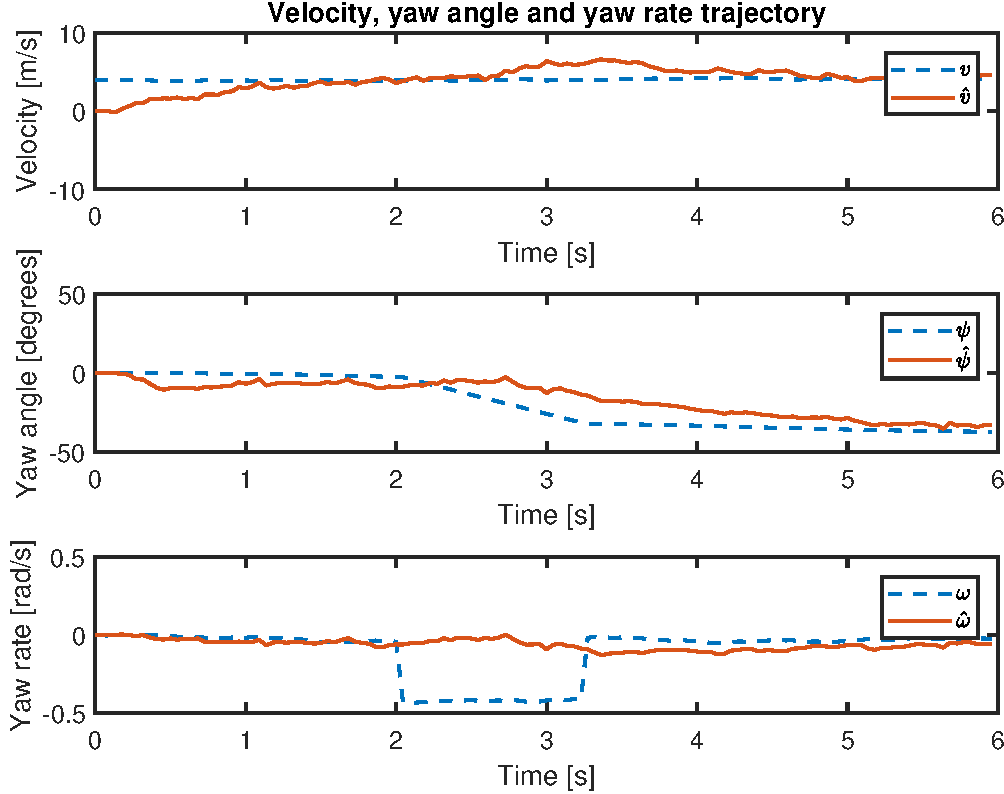
\includegraphics[width=0.8\textwidth]{ExampleTrajectory/13_MC_TrajOther}
	\caption{\label{fig:13trajectorycrossingroiother} One example of a trajectory from the Monte Carlo simulation in scenario 2 with setup 6.}
\end{figure}

\begin{figure}[!ht]
	\centering
	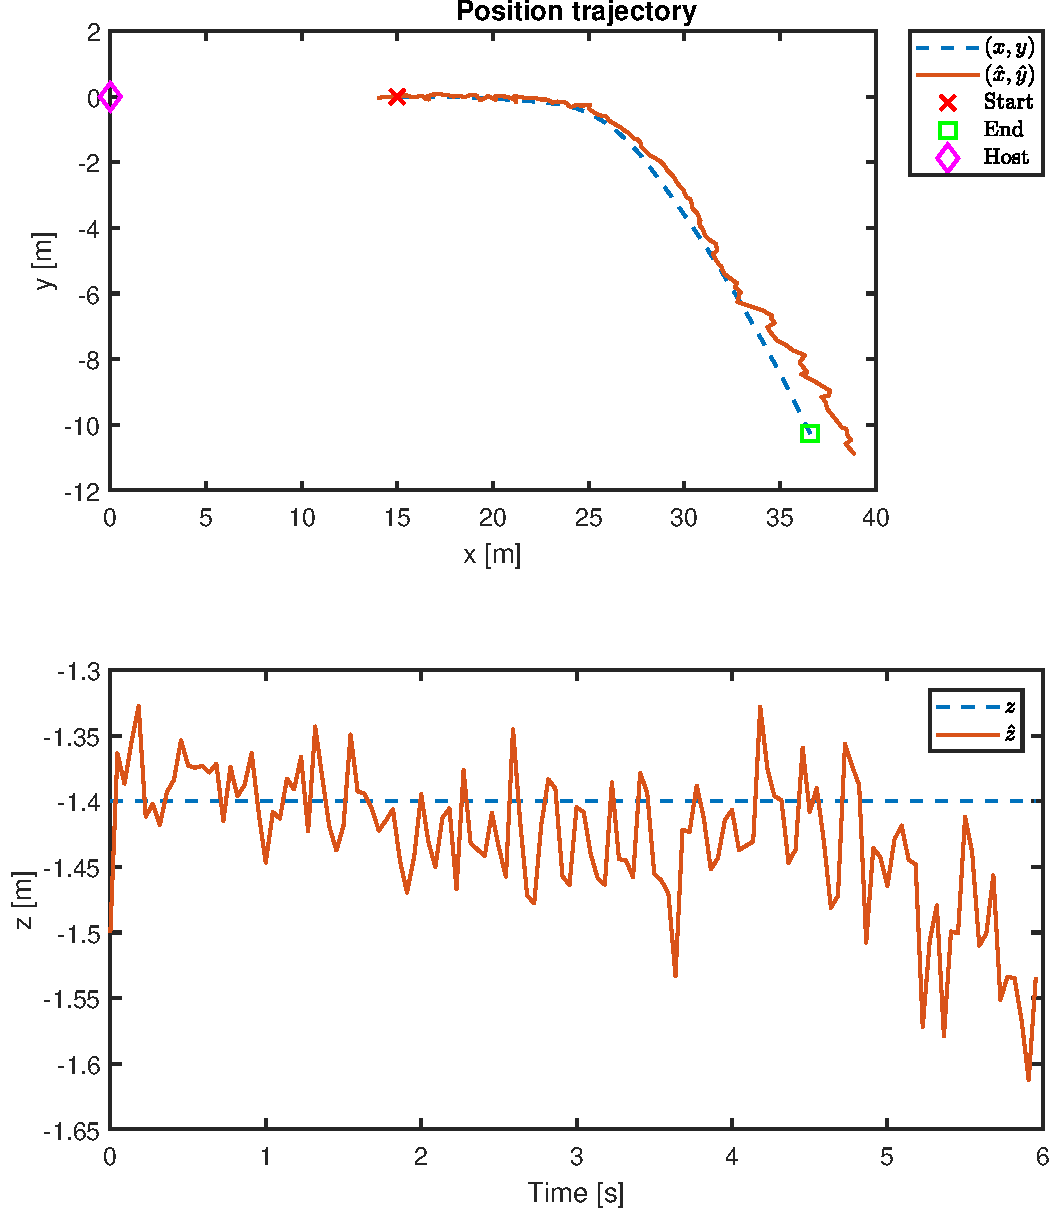
\includegraphics[width=0.6\textwidth]{ExampleTrajectory/23_MC_TrajPos}
	\caption{\label{fig:23trajectorycrossingroiangvelpos} One example of a trajectory from the Monte Carlo simulation in scenario 2 with setup 7.}
\end{figure}

\begin{figure}[!ht]
	\centering
	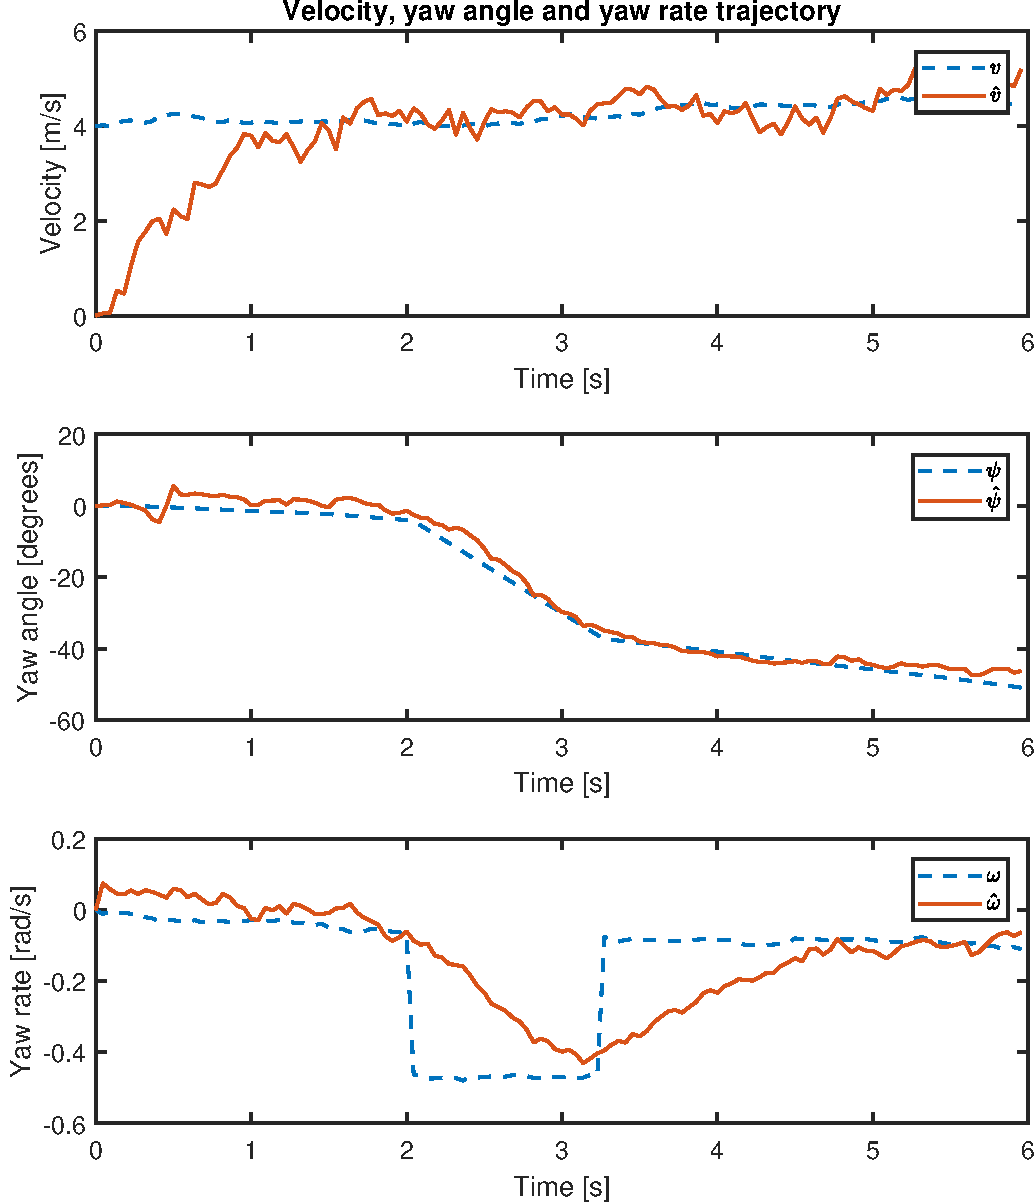
\includegraphics[width=0.5\textwidth]{ExampleTrajectory/23_MC_TrajOther}
	\caption{\label{fig:23trajectorycrossingroiangvelother} One example of a trajectory from the Monte Carlo simulation in scenario 2 with setup 7.}
\end{figure}

\begin{figure}[!ht]
	\centering
	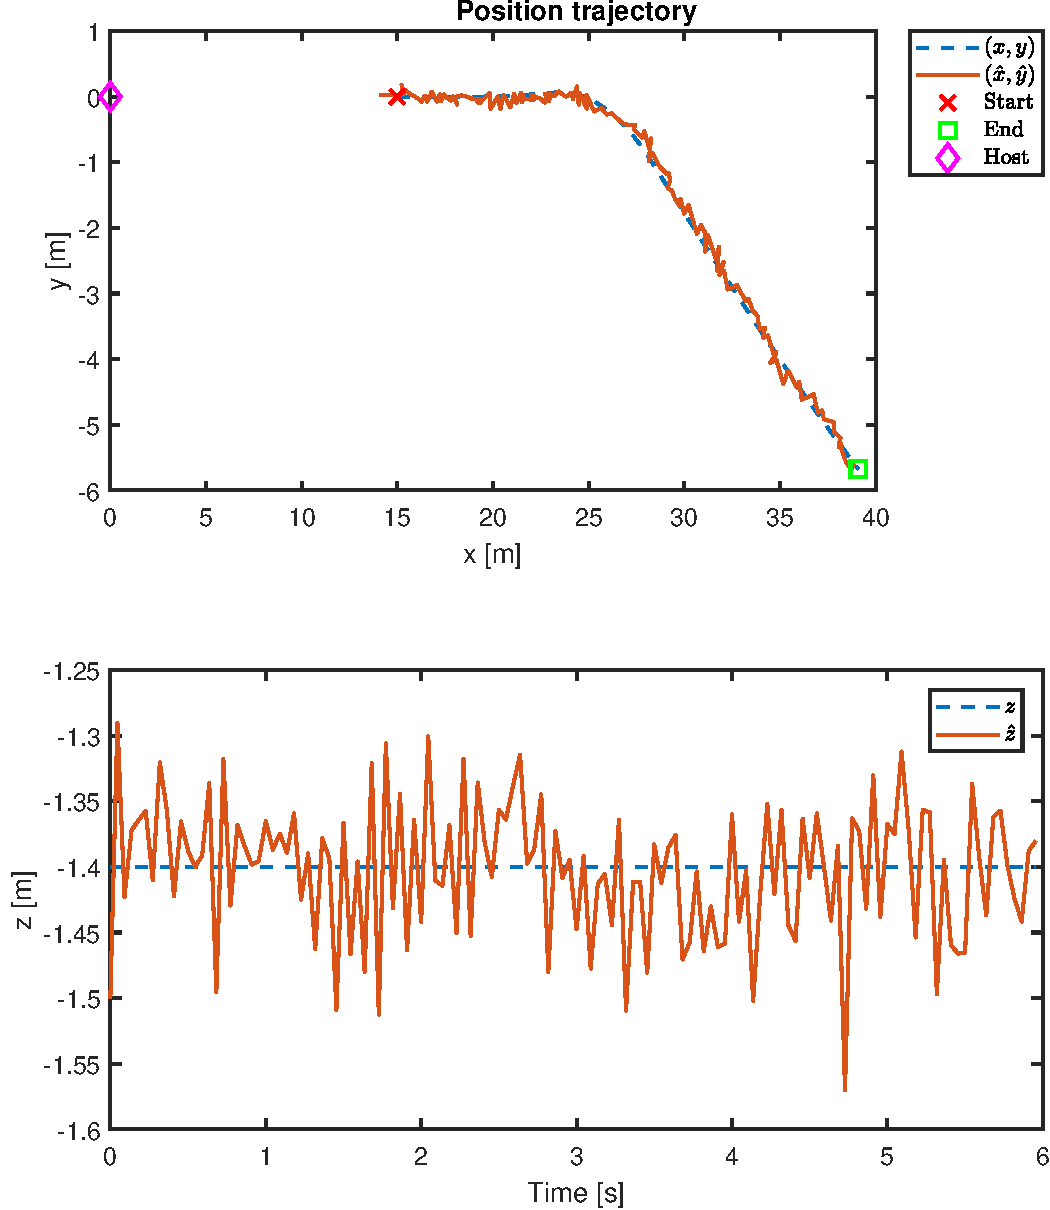
\includegraphics[width=0.6\textwidth]{ExampleTrajectory/29_MC_TrajPos}
	\caption{\label{fig:29trajectorycrossingroiangvelcornerpos} One example of a trajectory from the Monte Carlo simulation in scenario 2 with setup 10.}
\end{figure}

\begin{figure}[!ht]
	\centering
	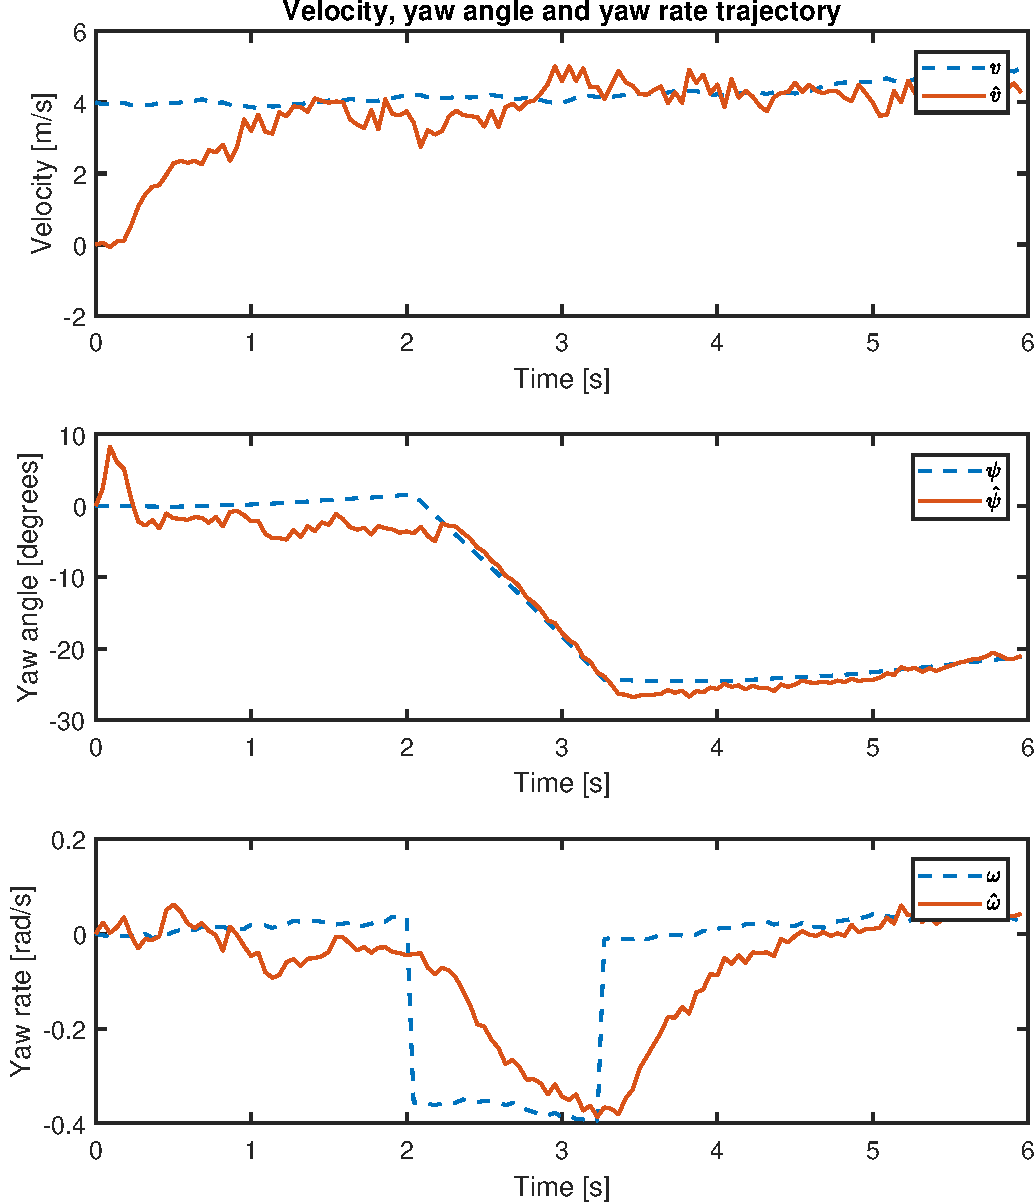
\includegraphics[width=0.5\textwidth]{ExampleTrajectory/29_MC_TrajOther}
	\caption{\label{fig:29trajectorycrossingroiangvelcornerother} One example of a trajectory from the Monte Carlo simulation in scenario 2 with setup 10.}
\end{figure}